\documentclass[a4paper]{article}
\usepackage{fullpage}
\usepackage{amsmath}
\usepackage{graphicx}
\usepackage[colorlinks]{hyperref}

\newcommand{\dd}{\text{d}}
\newcommand{\ii}{\text{i}}

\newcommand{\of}[1]{\left( {#1} \right)}
\newcommand{\fracd}[2]{\frac{\dd{}{#1}}{\dd{}{#2}}}

\newcommand{\dhref}[1]{\href{#1}{#1}}
\newcommand{\mailhref}[1]{\href{mailto:#1}{#1}}

\title{Final report on ``Heterogeneity of the Suprachiasmatic
Nucleus'' {\em BO 3612/2-1}}
\author{Hanspeter Herzel  \mailhref{h.herzel@biologie.hu-berlin.de},\\
        Grigory Bordyugov \mailhref{grigory.bordyugov@gmail.com}}
\date{\today}

\begin{document}
\maketitle

\begin{abstract}
  This DFG-supported project was aiming at uncovering the functional
  properties of circadian oscillator arrays of the SCN on different
  scales, ranging from single cell oscillations to ensemble effects.
  We report advances in several levels, including conceptual (phase of
  entrainment), single-cell mechanistic (molecular workings of
  regulatory gene networks), and tissue-wide (dynamics of oscillator
  ensembles). The common pattern appearing here is that a substantial
  number of circadian phenomena can be well understood in the
  framework of relatively simple mathematical models, parameterized by
  few parameters such as amplitude, period and phase of oscillations.
  Additionally, the collaboration with the lab of Prof Toru Takumi in
  RIKEN resulted in discovery of Choroid Plexus as another strong
  circadian oscillator in brain with the rhythmicity levels comparable
  with those of the SCN.
\end{abstract}

\tableofcontents

\section{Overview and main results}

\section{Main results: From modeling of single cell oscillations to
ensembles of neurons}

\subsection{Semi-automatic modeling for gene regulatory networks}
Within his masters dissertation, Matthew
Kondoff~\cite{kondoff2015modeling} looked at a way of automatically
generating computational models from human-readable description of
regulatory gene networks. His efforts resulted in an R package, with
the help of which a convenient way of numerical modeling was
providing, thus hiding the low-level nitty-gritty of translating the
network description into formulas and computer code.

\begin{figure}
\begin{center}
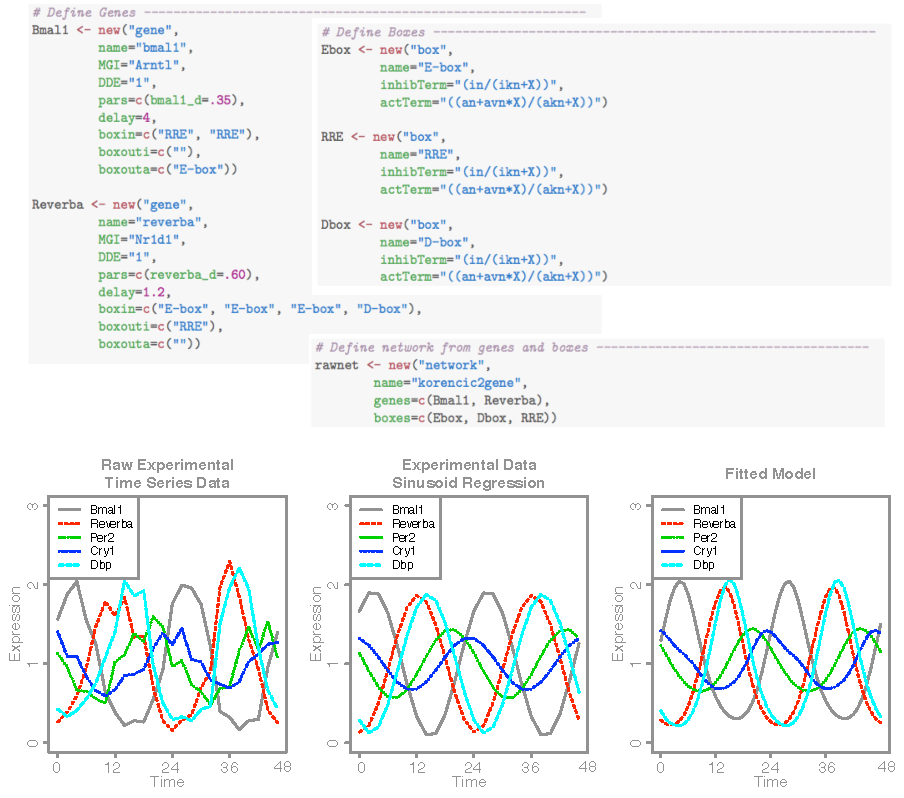
\includegraphics[width=\linewidth]{figures/matt/matt.pdf}
\end{center}
\caption{
Matt's figure
\label{fig::matt}
}
\end{figure}


Used~\cite{zhang2014circadian} microarray data to verify and fit the
parameters of the numerical model.


\section{Formal}

\subsection{Published and submitted papers}
papers
\cite{bordyugov2015tuning,schmal2015theoretical,kondoff2015modeling,schmal2017moran,wagner2017plant,myung2017choroid,schmal2017measuring}

\subsection{Student theses and projects}
Matthew Kondoff build a tool for automatically generating and
exploring regulatory networks of genes and fitted them to microarray
data of Hogenesch et al., which resulted in an R package
\cite{kondoff2015modeling}. Anna-Marie Finger and Lorena Sofia Lopez
Zepeda investigated the circadian regulation of immune system and
liver.  Sungsoo Lim and Marta del Olmo conducted computer-assisted
studies of entrainment phase in several models of circadian clock.



\section{Cooperation activities}

\subsection{Telecom conferences}
During the three years of the project, we maintained (mostly)
bi-weekly Skype conferences to synchronize our activities between
Tokyo and Berlin. The calls mainly included Christoph Schmal, Jihwan
Myung and GB.

\subsection{Visits between Japan and Germany}
The following visits between Tokyo and Berlin took place:
\begin{itemize}
  \item[-] Pia Rose visited Riken from Marth 2nd through April 25th 2015,
  \item[-] Christoph Schmal visited Riken from June 18th through July 3rd
  2014,
  \item[-] Hanpspeter Herzel visited Riken from July 17th through July
  20th 2014,
  \item[-] Toru Takumi visited the ITB in Berlin on three occasions from
  2014 through 2016,
  \item[-] GB visited Riken from February 10th through March 1st 2014.
\end{itemize}

\subsection{Conferences}
The results of the research on the project were presented at the
Gordon Conference on Chronobiology (Newport, RI in summer 2013, also
first contact with Jihwan Myung established there), at the conference
of the Japanese Society for Mathematical Biology (Osaka, Summer 2014),
at the congress of European Biological Rhythms Society in M\&unchen
(Fall 2014), and at the meeting of SRBR (summer 2016).

\bibliographystyle{vancouver}
\bibliography{jg-report}
\end{document}
